\documentclass[a4paper,12pt]{report}

\usepackage[utf8]{inputenc}
\usepackage[T1]{fontenc}
\usepackage{array}
\usepackage{amsmath}
\usepackage[english]{babel}
\usepackage{graphicx}
\usepackage[a4paper]{geometry}
\usepackage[colorlinks=true,urlcolor=blue,linkcolor=blue]{hyperref}
\usepackage{url}
\usepackage[nottoc,numbib]{tocbibind}
\usepackage{color}
\usepackage{epstopdf}
\usepackage{xcolor}
\usepackage[backend=biber,style=phys]{biblatex}
\usepackage[capbesideposition={right,center}]{floatrow}
\usepackage{lipsum}

\addbibresource{../Bibliography.bib}

\makeatletter
	\renewcommand{\thechapter}{\Roman{chapter}}
\makeatother

\floatsetup[table]{style=plaintop}

\begin{document}

\chapter{Dynamics and optical control of an individual Cr spin in a CdTe QD\label{CrDyn}}
	
	Lorem ipsum dolor sit amet, consectetur adipiscing elit. Curabitur tortor quam, imperdiet quis facilisis sed, fringilla a quam. Cras ante odio, hendrerit ac ante nec, cursus imperdiet urna. Mauris convallis ultricies purus, nec condimentum erat bibendum vel. Aliquam erat volutpat. Pellentesque condimentum, eros a consequat accumsan, turpis sem euismod nisi, sed fringilla quam turpis sit amet erat. Mauris dictum odio sed nisi dapibus, et molestie mauris rutrum. Praesent convallis dolor in nibh blandit bibendum. Quisque sit amet arcu consectetur lorem luctus venenatis nec quis dui. Aliquam erat volutpat. Aenean auctor elit nec tristique dignissim. Nulla massa mi, efficitur semper ex id, pretium eleifend massa. Vivamus sit amet orci scelerisque, gravida est ut, vulputate odio.
	
	\section{Resonant optical pumping and spin dynamics in a Cr doped QD}
	
		\subsection{Resonant optical pumping of the Cr spin\label{ResOptPump}}
		
	In order to study the dynamic of the X-Cr system, we need a dot presenting no contribution of the charged exciton in the spectra. Such a contribution would mean that supplementary carriers may be injected in the QD at random times, modifying its dynamics. Taking the spectra of QD2 on a large energy range, as presented on Fig.~\ref{PumpPres}, we see that this dot has a PL only at the X-Cr position, with no contribution of the other excitonic species. Even at high power, we were not able to observe a contribution of the biexciton. It is a good candidate for the study of the dynamics of a Cr coupled to a single exciton.
		
	\begin{figure}[h!]
	\begin{center}
		\includegraphics[width=14.7cm]{Pictures/PumpPres.png}
	\end{center}
	\caption{Low temperature PL spectra of QD2 exciton in lineraly polarized excitation and detection for B = 0T. No contribution of the charge excitons was found. Inset: Schematic of the energy levels in a Cr-doped QD and configuration of excitation/detection for resonant optical pumping. The ground states $S_z = 0$, $\pm1$ are split by the magnetic anisotropy $D_0 S_z^2$. In the excited state (X-Cr), the exchange interaction with the bright exciton ($|\pm1\rangle$) split the states $S_z = \pm1$.}
	\label{PumpPres}
	\end{figure}
	
	To initialize and read-out the Cr spin, we developed a two wavelengths pump-probe experiment. A circularly polarized single mode laser (\emph{resonant pump}) tuned on a X-Cr level is used to pump the Cr spin (i.e., empty the spin state under resonant excitation). Then, a second laser, tuned on an excited state of the QD (\emph{quasi-resonant probe}), injects excitons independently of the Cr spin $S_z$ and drives the Cr to an effective spin temperature where the three ground states $S_z=0$,$\pm1$ are populated~\cite{LafuenteCrQD}. By recording the PL of a X-Cr lines in circular polarization under this periodic sequence of excitation, we can monitor the time evolution of the population of a given Cr spin state.
	
	\begin{figure}[h!]
	\begin{center}
		\includegraphics[width=14cm]{Pictures/ExperimentSchema.png}
	\end{center}
	\caption{Schematic view of the micro-spectroscopy set-up used for the time-resolved optical pumping experiment. The monomode laser is a dye laser tuned on resonance with the studied dot transition, acting as the pump. The other dye laser is tuned on a resonant state at $E_{probe} = 2070$ meV, acting as the probe. Both beamsplitters are non-polarizing.}
	\label{PumpExpSetup}
	\end{figure}	
		
	Fig.~\ref{PumpExpSetup} shows our experimental set-up. Both of the continuous wave (CW) lasers passed through accousto-optic modulators, going on and off in turn. The modulators take about 10 ns to go from OFF to ON. Following them, a diaphragm is centered on the first diffraction spot created by the modulators. This creates a train of pulses of tunable duration and frequency, alternating between the pump and the probe. This two lasers are focused on the sample with a microscope objective. A SIL is also mounted on the sample surface, to increase the collection of photons emitted by the QD. The emitted light pass through a monochromator and is then collected with an avalanche photodiode.
	
	\begin{figure}[h!]
	\begin{center}
		\includegraphics[width=12cm]{Pictures/PumpResults.png}
	\end{center}
	\caption{(a) PL transients recorded in circular polarization on line (3) and on line (4) (as defined in the inset) under the resonant (pump on (1)) and quasi-resonant optical excitation sequences displayed at the bottom. Inset: PL of X-Cr and configuration of the resonant excitation and detection. (b) and (c): Energy detuning dependence of resonant PL intensity ($I_1$, at the beginning and $I_2$, at the end of the pump pulse) and of the corresponding normalized amplitude of pumping transient $\Delta I/I_2 = (I_1-I_2)/I_2$.}
	\label{PumpingExp}
	\end{figure}		
		
	The main features of the optical pumping experiment are presented in Fig.~\ref{PumpingExp}(a). The QD is excited on the high energy state of X-Cr with $\sigma-$ photons (X-Cr state $|S_z=-1,-1\rangle$). This excitation can only create an exciton in the dot if the Cr spin is $S_z=-1$. An absorption followed by possible spin-flips of the Cr in the exchange field of the exciton progressively decreases the population of $S_z=-1$. After this pumping sequence, the resonant pump is switched off and followed by the non-resonant probe.

	A clear signature of the optical pumping appears on the time evolution of the PL intensity of the low energy bright exciton line (4). The PL of this line during the probe pulse, recorded in opposite circular polarization with the resonant pump, depends on the population of $S_z=-1$. It strongly differs between the two pump-probe sequences where the resonant pump is on or off. The difference of intensity at the beginning of the probe pulse is a measurement of the efficiency of the pumping. The PL transient during the probe pulse corresponds to a destruction of the non-equilibrium population distribution prepared by the pump. As expected for an increase of the Cr spin temperature, the population of the ground spin state $S_z=0$ also decreases during the probe pulse. This decrease directly appears in the time evolution of the amplitude of the central X-Cr lines during the probe pulse (Det. (3) in Fig.~\ref{PumpingExp} (a)). The increase of the population of $S_z=0$ during the probe pulse shows that the population of $S_z=-1$ has been partially transferred to $S_z=0$ during the resonant pumping sequence. This transfer is controlled by the hole-Cr flip-flop via the interaction with an accoustic phonon, as described for the Mn in Sec.~\ref{RelaxMech}.
	
	A more direct way to probe the optical pumping speed and efficiency is to monitor the time evolution of the PL during the resonant excitation by the pump pulse. Under resonant excitation on the high energy X-Cr line, an exciton spin-flip with conservation of the Cr spin can produce a PL on the low energy line \cite{ClaireOptInit}. This experiment configuration is illustrated in the inset of Fig.~\ref{PumpPres}. In this process, the exciton flips its spin by emitting (or absorbing) an acoustic phonon. Such spin-flip is enhanced by the large acoustic phonon density of states at the energy of the inter-level splitting induced by the exchange interaction with the Cr spin which act as an effective magnetic field \cite{ExcSpinRelaxQD,ExcSpinDecay}. The resulting weak resonant PL signal depends on the occupation of the Cr state $S_z=-1$ and is used to monitor the time dependence of the spin selective absorption of the QD.
	
	The time evolution of the PL of the low energy line of X-Cr under an excitation on the high energy line is presented in Fig.~\ref{PumpingExp} (a) for two different pump-probe sequences: probe on and probe off. When the probe laser is on, a large effective Cr spin temperature is established before each pumping pulse. The amplitude of the resonant PL is maximum at the beginning of the pump pulse ($I_1$) and progressively decreases. A decrease of about 80\% is observed with a characteristic decay time in the tens of $ns$ range. When the probe laser is off, the initial amplitude of the PL transient during the pump pulse is significantly weaker. This decrease is a consequence of the conservation of the out of equilibrium Cr spin distribution during the dark time between two consecutive pumping pulses.
	
	The steady state resonant PL intensity reached at the end of the pump pulse ($I_2$) depends on the optical pumping efficiency which is controlled by the ratio of the spin-flip rate for the Cr spin in the exchange field of the exciton and the relaxation of the Cr spin in the empty dot. However, even with cross-circularly polarized excitation/detection, this steady state PL can also contain a weak contribution from an absorption in the acoustic phonon sideband of the low energy line~\cite{BesombesAccPhon}. Fig.~\ref{PumpingExp} (b) presents the amplitude of the resonant PL detected on the low energy line for a detuning of the pump around the high energy line. A resonance is observed in the initial amplitude $I_1$ of the PL. It reflects the energy dependence of the absorption of the QD. A small decrease of the steady state PL $I_2$ is also observed at the resonance. As displayed in Fig.~\ref{PumpingExp} (c), the corresponding normalized amplitude of the pumping transient, $(I_1-I_2)/I_2$, presents a clear resonant behaviour demonstrating the excitation energy dependence of the optical pumping process. The width of the resonance ($\sim 100\mu eV$) is the width of the QD's absorption broadened by the fluctuating environment~\cite{SubnanoSpectralDiff}.

	\begin{figure}[h!]
	\caption{Optical pumping under a CW probe at $E = 2004$ meV. (a) Pumping on line (1) and detecting on line (4). (b) Pumping on line (4) and detecting on line (1).}
	\label{ContProbe}
	{\begin{center}
		\includegraphics[width=11cm]{Pictures/ContProbe.eps}
	\end{center}}
	\end{figure}

	The experiment was also done without modulating the probe (probe ON all the time). We did the experiment in two configuration, presented on Fig.~\ref{ContProbe}: either pumping on line (1) (high energy) and detecting on line (4) (low energy), or the opposite. When the pump pulse is turned on the high energy peak, we can see the same transients as shown in Fig.~\ref{PumpingExp}: a first, quick increase followed by a slower decrease. The amplitude of the pumping transient is however smaller, due to the pumping state being continuously heated and thus destroyed. When the pulse is turned off, the  PL decreases quickly, followed by a slow increase during about 200 ns before coming back at the it has before the pumping. This transient is the same as the one observed on the probe pulse in Fig.~\ref{PumpingExp}.
	
	The complimentary evolution happens when we pump on the line (4) and detect on line (1). In this case, when the pumping laser is turned on, we first observe a decrease about 100 ns long. The PL intensity then stabilize before diminishing slightly when the pump pulse finish, and then increasing slowly in a 200 ns timescale. The first decrease correspond to the establishment of the pumped state: the high energy state is emptied to fill the low energy one. Since there is no mechanism allowing the system to come back in the high energy state, it then stays empty for the duration of the pumping pulse. However, since the probe laser stays on even during the pump pulse, the state is still populated by it, and so some photons are still detected during this time. As before, the increase after the end of the pumping correspond to the destruction of the nonequilibrium population distribution established during the pumping pulse, and the repopulation of the emptied states.
	
	\begin{figure}[h!]
	\begin{center}
		\includegraphics[width=14.8cm]{Pictures/PWProbe.eps}
	\end{center}
	\caption{PL transients measured on line (4) while pumping on line (4) at $P_{pump} = 250$ $\mu$W (red) or without pumping (dark). (a) $P_{probe} = 125 $ $\mu$W. (b) $P_{probe} = 250 $ $\mu$W. (c) $P_{probe} = 500 $ $\mu$W.}
	\label{PWProbe}
	\end{figure}
	
	We studied evolution of the quantum dot PL under variation of the probe laser power. The results are presented on Fig.~\ref{PWProbe}. The first noticeable evolution is the intensity increase, proportional to the increase of the probe power. A higher power lead to a higher probability of injecting an exciton in the QD. Therefore, more photon will be emitted by the dot, proportionally to the laser power, as long as there is no contribution of the biexciton.
	
	More interestingly, we observe that the speed of this spin heating process depends on the intensity of the probe laser. The probe pulse last for about 500 ns, and, for a laser power of 125 $\mu$W, the nonequilibrium population distribution is not completely destroyed at the end of it (Fig.~\ref{PWProbe} (a)). The transient reduces to about 200 ns for a laser power of 500 $\mu$W. This speeding of the heating process is also controlled by the higher rate of carriers injection. The heating is done by the interaction between the excitons and the Cr spin. The probe inject excitons at high energy in the QD, interacting with the Cr independently of its spin state. A higher number of injected high energy carriers therefore lead to a quicker destruction of the nonequilibrium state created by the pump pulse.
	
	\begin{figure}
	\fcapside{\caption{Detail of the PL transient measured during the resonant pump pulse for a power $P_{probe} = 250$ $\mu$W. The exponential fit (green) gives a characteristic time of $\tau_{pump} = 60$ ns. The inset presents the evolution of $\tau_{pump}$ as a function of the pumping laser power.}\label{PWPump}}
	{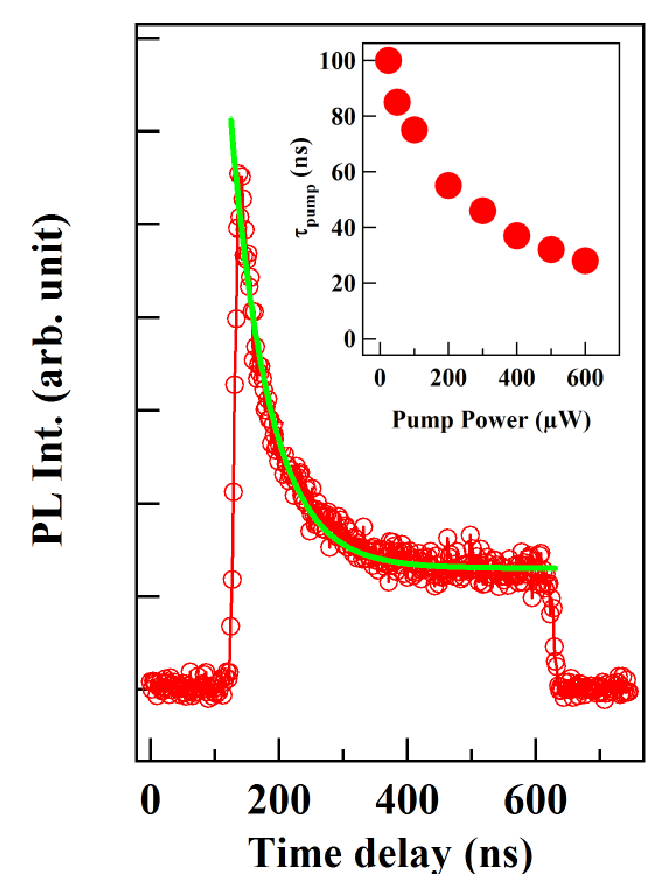
\includegraphics[width=7cm]{Pictures/PWPump.eps}}
\end{figure}
	
	Injecting carriers at the energy of a given transition at a higher rate also helps pumping it quicker. The results of such an experiment are presented on Fig.~\ref{PWPump}. As expected for a spin optical pumping process, the characteristic time of the PL transient decreases with the increase of the pump laser intensity (inset of Fig.~\ref{PWPump})~\cite{ClaireOptInit}. This acceleration of the pumping is also due to the higher probability of carriers to be in the quantum dot. The system is pumped in a given when interacting with carriers with right spin and at the energy of the transition associated with the Cr spin state. A higher injection rate of carrier at this particular energy increase the probability of interacting with the Cr on the right spin state, and thus pump the system quicker.
	
%	\begin{figure}
%	{\caption{(a) Detail of the PL transient measured during the resonant pump pulse for a power $P_{probe} = 250$ $\mu$W. The exponential fit (green) gives a characteristic time of $\tau_{pump} = 60$ ns. The inset presents the evolution of $\tau_{pump}$ as a function of the pumping laser power. (b) Evolution of the normalized intensity $\Delta I/I$ as a fuction of the pump power.}\label{PWPump}}
%	{\includegraphics[width=12cm]{Pictures/PWPump+D1.eps}}
%	\end{figure}
%	
%	A systematic study of the normalized intensity as a function of the pumping power is presented on Fig.~\ref{PWPump} (b). We were not able to measure it for pump power higher than 200 $\mu$W because the starting time of the accousto-optic modulator was cutting the beginning of the transient and thus making it appears less intense than it really is. However, we can see that the transient normalized intensity stabilized between 3.5 and 4. This stabilization is expected when reaching high pumping power. The intensity of the detected 
	
%	For most of the experiments, we chose a pump power and a probe power of 250 $\mu$W. At this power, the nonequilibrium state is created (pump pulse) or destroyed (probe pulse in a few hundreds of nanoseconds, but with a transient slow enough to be easily distinguished and measured. This way, we keep our pulse duration 	
	
		
		\subsection{Dynamics of the Cr spin under optical excitation}
		
%			\subsubsection*{Autocorrelation and cross-correlation}		
		
		We performed auto-correlation of the photoluminescence (PL) intensity emitted by individual lines of an isolated Cr-doped QD to probe the dynamics of the magnetic atom under continuous wave (CW) optical excitation. A Hanbury Brown and Twiss (HBT) setup was used for this purpose. In these start-stop experiments, the detection of the first photon indicates by its energy and polarization that the Cr spin has a given orientation. The probability of detection of a second photon with the same energy and polarization is proportional to the probability of conserving this spin state. The time evolution of the auto-correlation is a probe of the spin dynamics in the Cr-doped QD.
	
	\begin{figure}[h!]
	\fcapside{\caption{Auto-correlation of the PL intensity collected in circular polarization on the X-Cr lines (1), (4) and (5) (as defined in Fig.~\ref{PumpingExp}) and compared with the auto-correlation of the exciton in a non-magnetic QD (black line). The curves are shifted for clarity. For line (1), the auto-correlation is also recorded under a transverse magnetic field (blue line).}\label{AutocorExpCr}}	
	{\begin{center}
		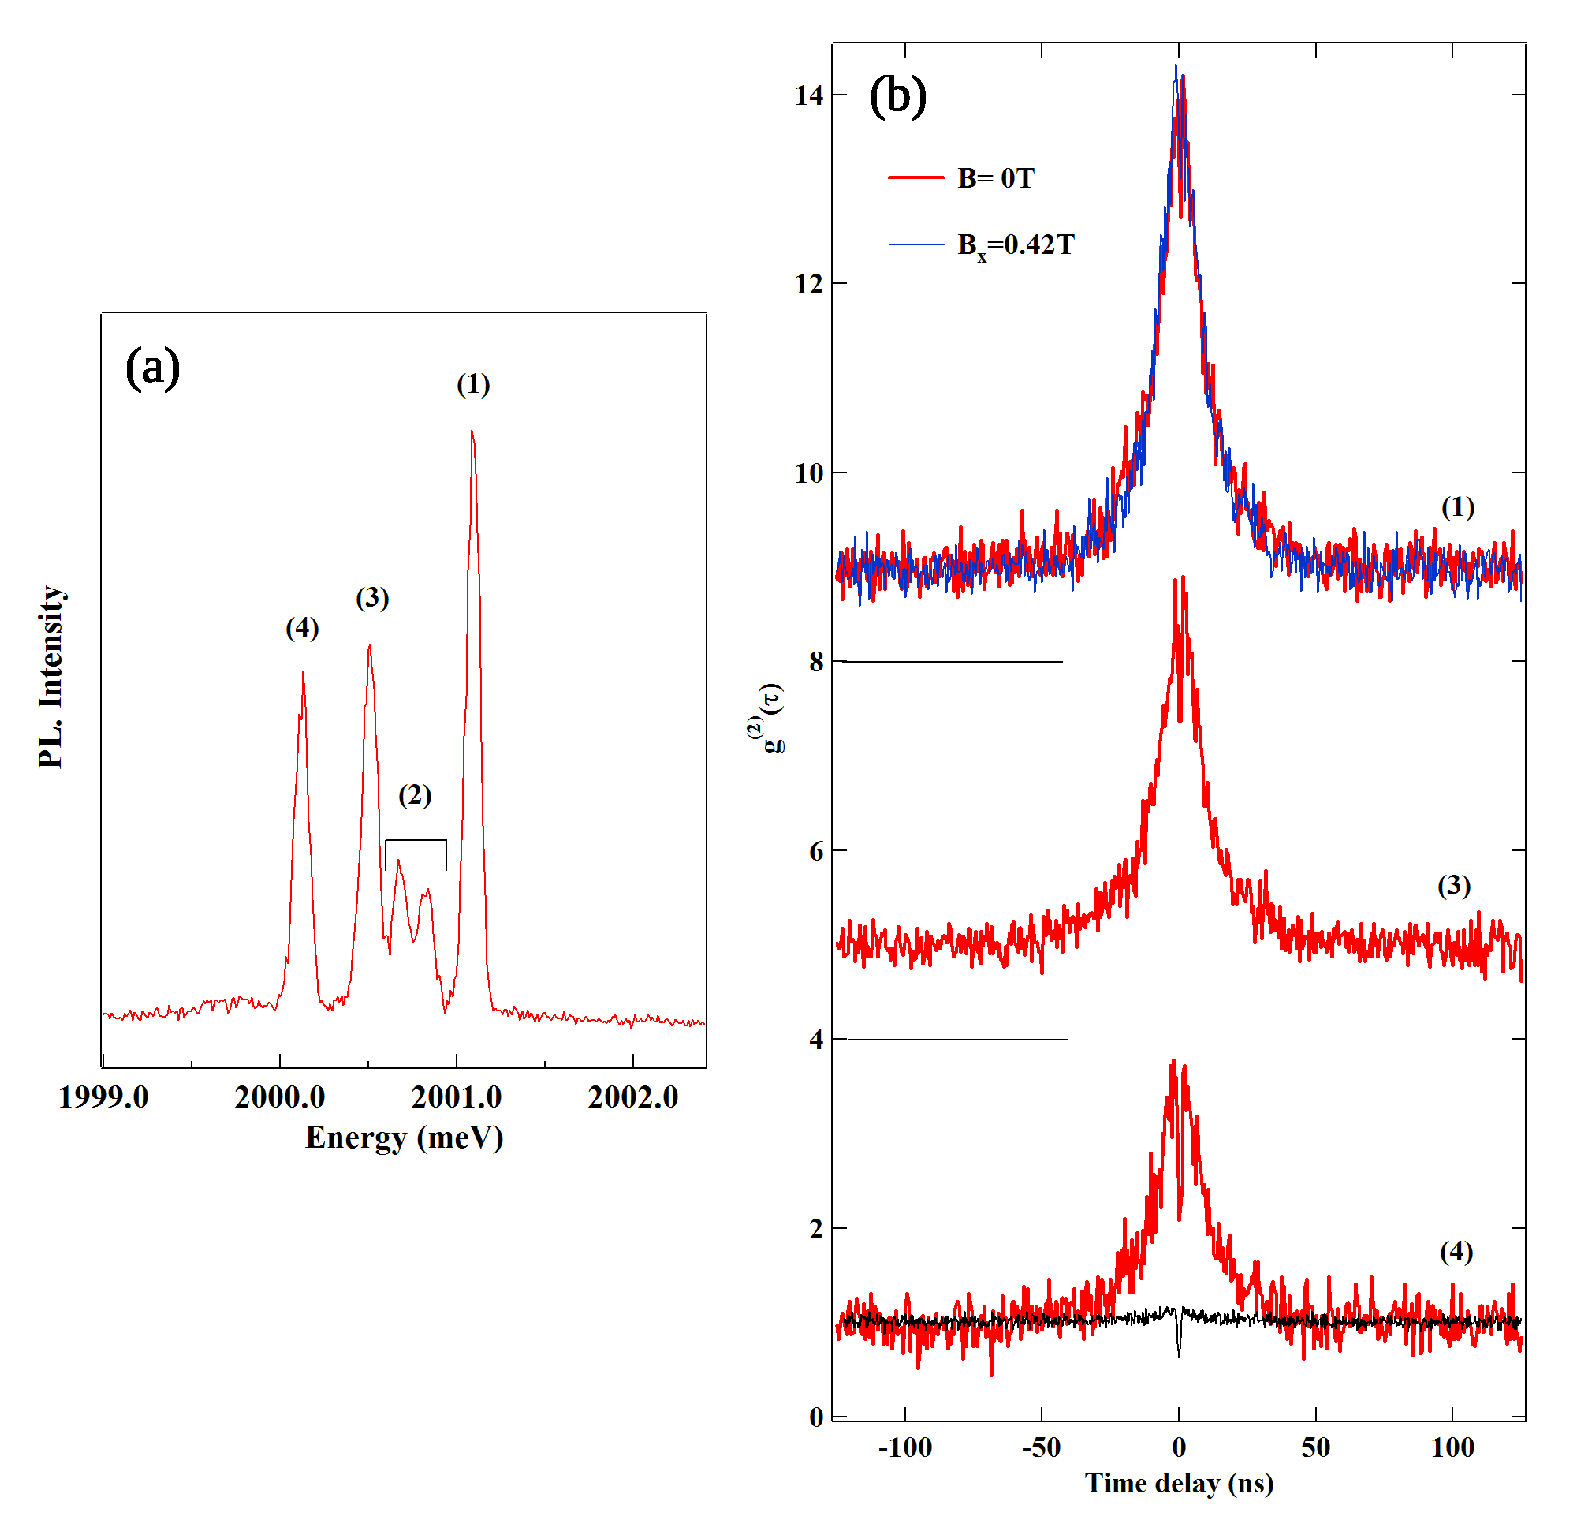
\includegraphics[width=7cm]{Pictures/AutocorPeaks.eps}
	\end{center}}
	\end{figure}	
	
			To observe the time fluctuations of the Cr spin under CW optical excitation, we used the statistics of time arrivals of the photons emitted by a Cr-doped QD given by the second order correlation function g$^{(2)}(\tau)$ of the PL intensity. Fig.~\ref{AutocorExpCr} shows g$^{(2)}(\tau)$ for the lines (1), (4) and (5) recorded in circular polarization. These signals are compared with the auto-correlation obtained for the PL of a non-magnetic QD which is characteristic of a single-photon emitter with a dip (anti-bunching) at short delays. The width of the anti-bunching is given by the lifetime of the emitter and the generation rate of excitons and its depth is limited by the time resolution of the HBT setup. As illustrated in Fig.~\ref{AutocorExpCr}, typical non-magnetic CdTe/ZnTe QDs do not present any significant bunching induced by charge fluctuations \cite{QDAutocor,IndistPhoton}. A similar auto-correlation on a X-Cr PL line still presents a reduced coincidence rate near zero delay, but it is mainly characterized by a large photon bunching with a full width at half maximum (FWHM) in the 20 ns range. This large bunching reflects an intermittency in the emission of a given line of the QD coming from fluctuations of the Cr spin in a 10 ns timescale as it will be confirmed by cross-correlation measurements.

		The amplitude of the bunching reaches 5 for line (1) and is slightly weaker for the lower energy lines. In a simple picture of blinking where the selected QD line can be either in a state ON or OFF, the amplitude of the bunching is given by $\Gamma_{OFF}/\Gamma_{ON}$, ratio of the transition rates from OFF to ON, $\Gamma_{ON}$, and from ON to OFF, $\Gamma_{OFF}$ \cite{SubnanoSpectDiff}. An amplitude of bunching larger than 1 is then expected in a multilevel spin system where, after a spin relaxation, multiple spin-flips are usually required to come back to the initial state ($\Gamma_{ON}<\Gamma_{OFF}$). Let us finally note that the bunching signal is not affected by a weak transverse magnetic field ($B_x=0.42$ T in Fig.~\ref{AutocorExpCr}). This confirms the presence of a large strain induced magnetic anisotropy $D_0$ which splits the Cr and X-Cr states and blocks their precession in a magnetic field.
		
	\begin{figure}[h!]
	\fcapside{\caption{Auto-correlation of the PL intensity recorded in circular polarization on the high energy X-Cr line (1) for different excitation powers. The inset shows the corresponding FWHM of the bunching signal versus excitation power.}\label{AutocorPW}}	
	{\begin{center}
		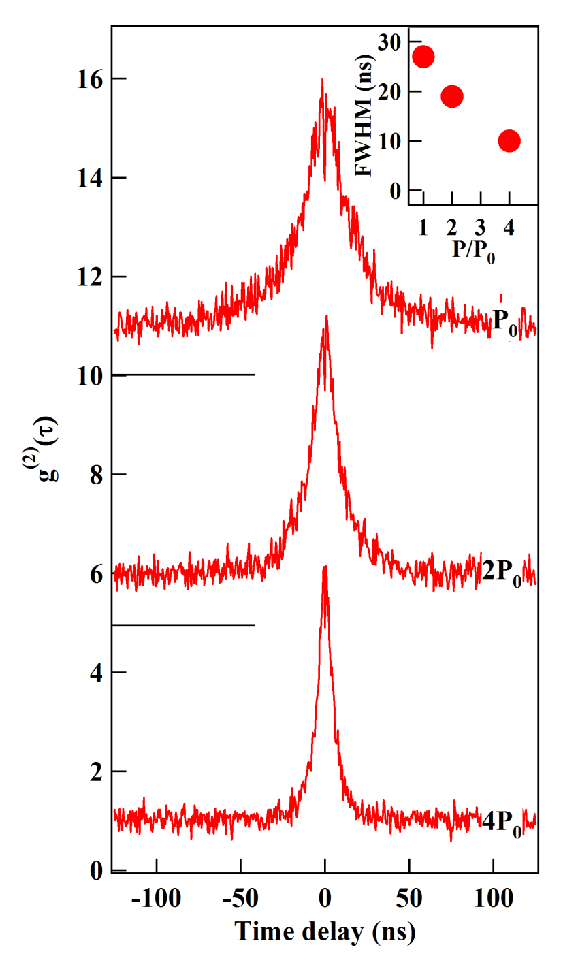
\includegraphics[width=7cm]{Pictures/AutocorPw.eps}
	\end{center}}
	\end{figure}
	
	One should note that the observed spin dynamics depends on the optical excitation power. Increasing the excitation power significantly reduces the width of the bunching (Fig.~\ref{AutocorPW}), linked to an increase of the Cr spin fluctuations. Within the X-Cr complex, the electron-Cr exchange interaction and the hole-Cr exchange interaction in the presence of heavy-hole/light-hole mixing can both induce spin-flips of the Cr. Though weak, the probability of such spin flips increases with the occupation of the QD with an exciton and dominates the spin dynamics in the high excitation regime required for the photon correlation measurements.
	
	\begin{figure}[h!]
	\begin{center}
		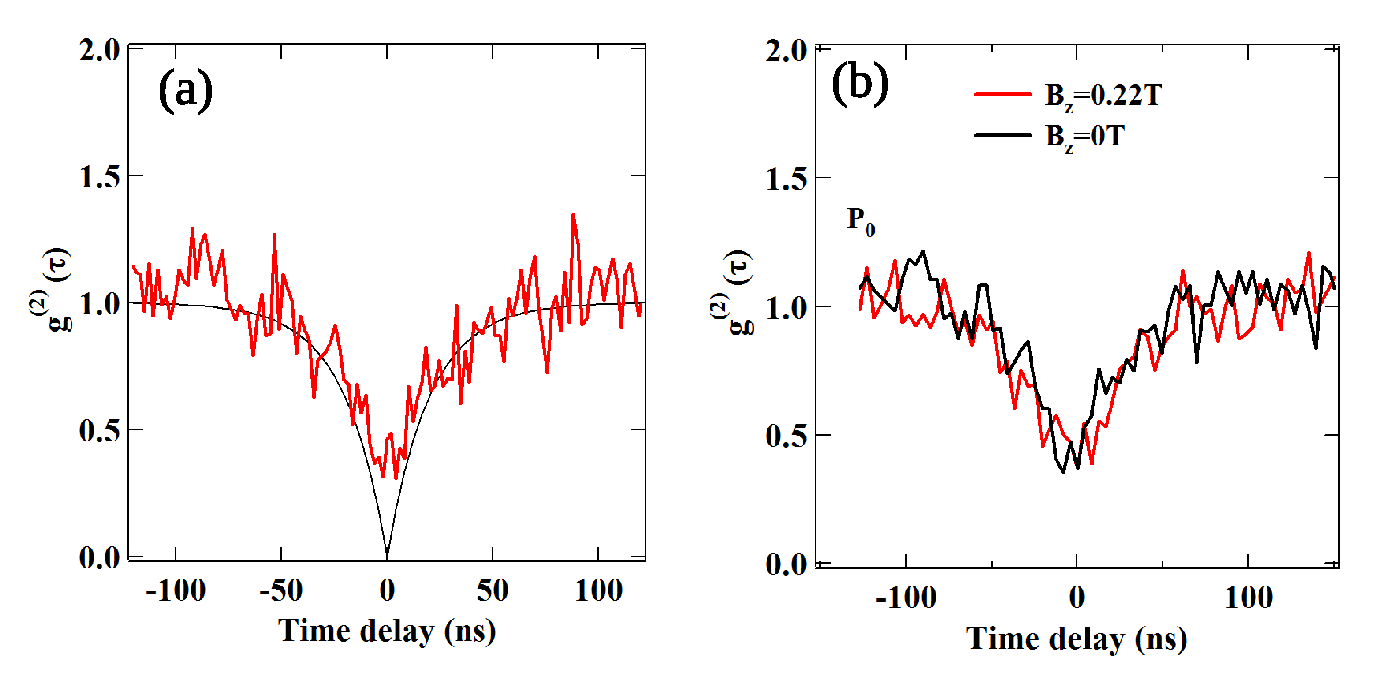
\includegraphics[width=10cm]{Pictures/CrosscorFit+B.eps}
	\end{center}
	\caption{(a) Correlation signal of the PL intensity of lines (1) and (4) recorded in the same circular polarization (cross-correlation) for three different excitation powers. The curves are shifted for clarity. The black line is an exponential fit with a characteristic time $\tau=20$ ns. (b) Longitudinal magnetic field dependence of the cross-correlation signal obtained at low excitation power.}
	\label{Crosscor}
	\end{figure}
	
	The excitation power dependence shows that the measured width of the bunching is not limited by the intrinsic Cr spin relaxation time $\tau_{Cr}$. This gives a lower bound for $\tau_{Cr}$ in the 20 ns range. A shorter value would impose, at low excitation intensity, faster spin fluctuations than observed experimentally. The Cr spin relaxation time is ultimately controlled by the interaction with acoustic phonons and could depend on the optical excitation through the generation of non-equilibrium acoustic phonons during the relaxation of injected carriers~\cite{PhotocarrierSpinHeat,EnTransPhotocarrierMn}. It is however expected to be longer than the observed dynamics~\cite{CaoSpinPhonCoupl} and cannot be determined with these measurements which require a large photon count rate.
	
	To analyze more in detail the spin relaxation channels, cross-correlation measurements were performed on the PL emitted by the high energy and the low energy lines in the same circular polarization. The cross-correlation shows a large anti-bunching with a FWHM in the 10 ns range and g$^{(2)}$(0)$\approx$0.3 (Fig.~\ref{Crosscor}(a)). Whereas the auto-correlation probes the probability for the Cr spin to be conserved, this cross-correlation is a probe of the spin transfer time between the spin states $S_z=+1$ and $S_z=-1$. As for the auto-correlation, the cross-correlation strongly depends on the excitation power. At weak excitation, a spin transfer time of about 20 ns is observed. It is accelerated with the increase of the excitation power (Fig.~\ref{Crosscor}(a)). This transfer time could be controlled by anisotropic in-plane strain which couples Cr spin states separated by two units through an additional term $E(S_x^2-S_y^2)$ in the Cr fine structure Hamiltonian~\cite{LafuenteCrQD}. However, even at low excitation power, the measured transfer time is not affected by a longitudinal magnetic field (Fig.~\ref{Crosscor}(b)). This shows that for such QD the strain anisotropy term $E$ is weak and is not the main parameter controlling the transfer time between the states $S_z=\pm1$. The spin transfer time is dominated by spin-flips induced by the exciton/Cr interaction.
	
%			\subsubsection{Relaxations through dark states}
%			
%		Lorem ipsum dolor sit amet, consectetur adipiscing elit. Curabitur tortor quam, imperdiet quis facilisis sed, fringilla a quam. Cras ante odio, hendrerit ac ante nec, cursus imperdiet urna. Mauris convallis ultricies purus, nec condimentum erat bibendum vel. Aliquam erat volutpat. Pellentesque condimentum, eros a consequat accumsan, turpis sem euismod nisi, sed fringilla quam turpis sit amet erat. Mauris dictum odio sed nisi dapibus, et molestie mauris rutrum. Praesent convallis dolor in nibh blandit bibendum. Quisque sit amet arcu consectetur lorem luctus venenatis nec quis dui. Aliquam erat volutpat. Aenean auctor elit nec tristique dignissim. Nulla massa mi, efficitur semper ex id, pretium eleifend massa. Vivamus sit amet orci scelerisque, gravida est ut, vulputate odio.
%	
%	\begin{figure}[h!]
%	\begin{center}
%		\includegraphics[width=10cm]{Pictures/FillingPicture.png}
%	\end{center}
%	\caption{Excitation power variations of the spectra and plot of the intensity of each peak}
%	\label{CrSpectraPwExp}
%	\end{figure}
%	
%	In order to study the different relaxation path of the system, probing of the emission evolution under excitation power was realized, reported on Fig.~\ref{CrSpectraPwExp}. As expected, the PL is becoming more intense with the augmentation of the excitation laser, since more exciton are produced and thus injected in the quantum dot. However, this power augmentation response is not the same for each of the peaks. The two central peaks, associated with the $|0\rangle$ states, start at about twice the intensity of the $|\pm1\rangle$ peaks for the most intense one, seemingly never reaching their maximum under our power range. However, when lowering the excitation power, they diminish quickly, and even seems to disappear at low energy, when exterior peaks still show luminescence. Plotting this evolution shows that the two central peaks exhibit a super-linear evolution. On the other side, the exterior peaks begin by rising in intensity before diminishing in a sub-linear fashion. This is coherent with the usual picture, where high power populating preferentially X$^2$-Cr states, while low power populates preferentially X-Cr states~\cite{??}. Finally, one can notice that the dark exciton exhibit the same behaviour, but the maximum emission intensity is at slightly lower power than the $|\pm1\rangle$.
%
%	\begin{figure}[h!]
%	\begin{center}
%		\includegraphics[width=10cm]{Pictures/FillingPicture.png}
%	\end{center}
%	\caption{Power variation simulation}
%	\label{CrSpectraPwMod}
%	\end{figure}
%	
%	The results of this evolution are well reproduced by our spin effective Hamiltonian, using the parameters found for the dot from the magneto-optics and the linear polarization fitting. The model results are presented in Fig.~\ref{CrSpectraPwMod}. [NOT SURE, TO BE REDISCUSSED]The super-linear behaviour of the central peaks can be explained by the proximity of dark exciton states. High power excitation can unlock radiative recombination path to states remaining non-radiative at low excitation power~\cite{PwSuperLinInc}. Such states linked to the $|0\rangle$ state make the emission on its peaks present a super-linear behaviour when excited at high power.
%
%		\subsection{Model of the spin dynamics}	
%
%	\begin{figure}[h!]
%	\begin{center}
%		\includegraphics[width=10cm]{Pictures/FillingPicture.png}
%	\end{center}
%	\caption{Simulation of autocorrelation on each peak and cross-correlation $|+1\rangle$ to $|+1\rangle$}
%	\label{SimulCRossAuto}
%	\end{figure}			
%		
%	To identify the main contribution to the observed spin fluctuations, we modelled the auto-correlation of the PL of X-Cr using the full spin level structure of a Cr-doped QD. We calculated the time evolution of the population of the twenty X-Cr states in the excited state of the QD and five Cr states in the ground state by solving numerically the master equation for the corresponding 25 x 25 density matrix $\rho$. The time evolution of the density matrix including relaxation and dephasing processes in the Lindblad form is given by $\partial \rho/\partial t=-i/\hbar[{\cal H},\rho]+L\rho$ where ${\cal H}$ is the Hamiltonian of the complete system ($X$-Cr and Cr) and $L\rho$ describes the coupling or decay channels resulting from an interaction with the environment \cite{SpinQJumps,ephBroad}. The energy levels of the Cr are controlled by the magnetic anisotropy $D_0S_z^2$. The X-Cr Hamiltonian, presented in Ref.\cite{LafuenteCrQD}, contains the energy of the Cr spin states, the carriers-Cr exchange interactions, the electron-hole exchange interaction in a confining potential of low symmetry and the structure of the valence band including heavy-hole/light-hole mixing. $D_0$ in the Cr Hamiltonian and the parameters in the X-Cr Hamiltonian cannot be precisely extracted from the zero magnetic field PL (Fig.~\ref{DotSpectra}(a)). For a qualitative description of the observed spin dynamics, we use in the model typical Cr-doped QD parameters extracted from magneto-optics measurements presented in Ref. \cite{LafuenteCrQD}. These parameters give a X-Cr splitting and a dark/bright excitons mixing similar to the one observed in the QD discussed in this article.
	
		\subsection{Cr spin relaxation in the dark}

		Using resonant optical pumping technique presented in Sec.~\ref{ResOptPump} to prepare and read-out the Cr spin, we performed pump-probe experiments to observe its relaxation time in the absence of carriers (Fig.~\ref{RelaxDark}). A non-equilibrium distribution of the Cr spin population is prepared with a circularly polarized resonant pump pulse on the high energy X-Cr line. The pump laser is then switched off, and switched on again after a dark time $\tau_{dark}$. The amplitude of the pumping transient observed on the resonant PL of the low energy line depends on the Cr spin relaxation during $\tau_{dark}$. As presented in Fig.~\ref{RelaxDark} (b), the amplitude of the transient is fully restored after a dark time of about 10 $\mu$s showing that after this delay the Cr spin is in equilibrium with the lattice temperature (T=5 K). Let us note, however, that the initial amplitude of the pumping transient in this case is weaker than the one observed after a non-resonant probe pulse (Fig.~\ref{PumpingExp} (a)). This means that the non-resonant optical excitation drives the Cr spin to an effective temperature much larger than the lattice temperature.
		
	\begin{figure}[h!]
	\begin{center}
		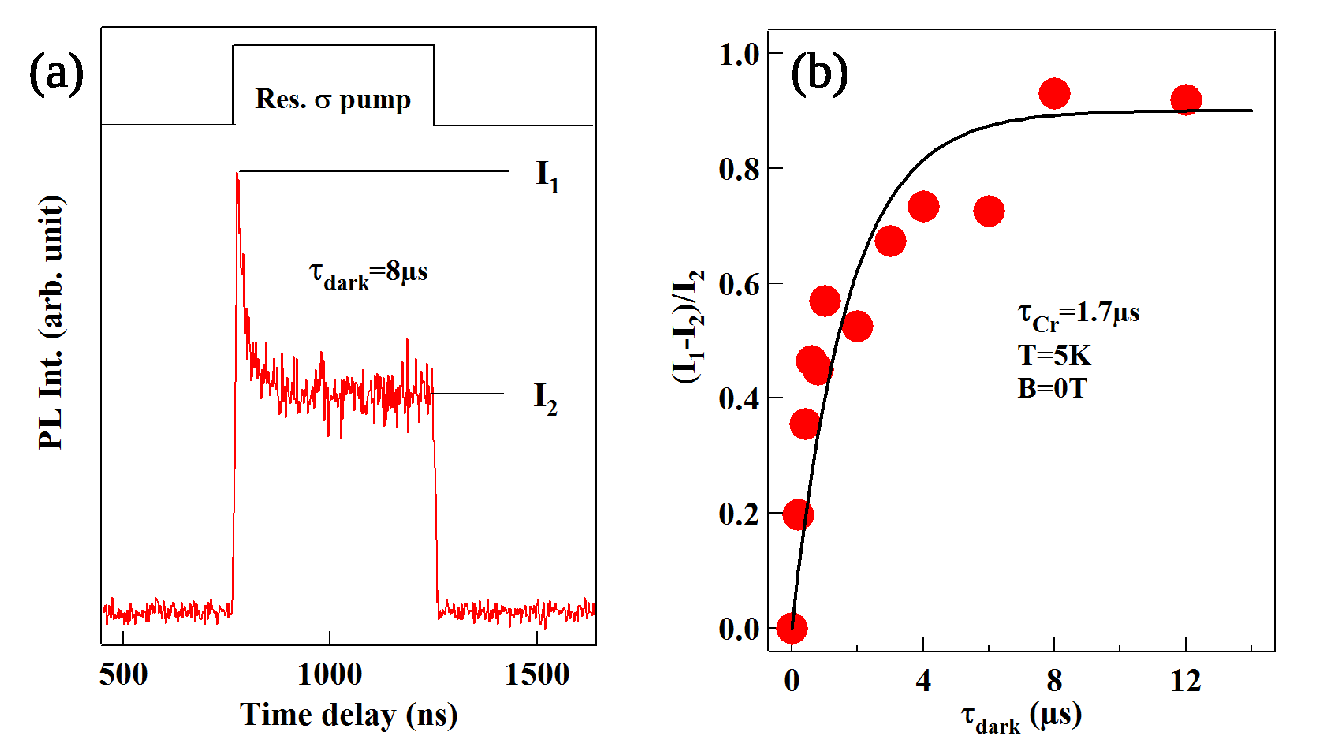
\includegraphics[width=12cm]{Pictures/RelaxDark.eps}
	\end{center}
	\caption{(a) Time evolution of the PL intensity of line (4) of X-Cr under resonant excitation on line (1) with a circularly polarized excitation pulse. (b) Evolution of the amplitude of the pumping transient $\Delta I/I_2$ as a function of the dark time between the excitation pulses. The black line is an exponential evolution with a characteristic time $\tau_{Cr}=1.7$ $\mu$s}
	\label{RelaxDark}
	\end{figure}		
		
	From the time delay dependence of the amplitude of the transient, we deduce a Cr relaxation time $\tau_{Cr}\approx1.7$ $\mu$s at B$=0$ T and T$=5$ K. For such neutral QD and in the absence of optical injection of carriers, this spin relaxation is likely to be controlled by the spin-lattice interaction. Despite the large spin-phonon coupling expected for this magnetic atom with an orbital momentum and a strain induced spin splitting in the meV range~\cite{LafuenteCrQD}, the Cr spin relaxation time remains in the $\mu s$ range. This spin memory is long enough for a practical use of Cr in an hybrid spin nano-mechanical system and could even be improved in different QDs structures with weaker biaxial strain~\cite{LucienSFD}, lower magnetic anisotropy splitting and consequently less coupling with acoustic phonons \cite{CaoSpinPhonCoupl}.
	
	The Cr spin-flip time found for a relaxation in the dark (microseconds range) is a lot longer than the one found under optical excitation (tens of nanosecond range, see Sec.~\ref{ResOptPump}). The fast Cr spin-flip under optical excitation can be due to the interaction with carriers (exchange induced Cr spin flips~\cite{CaoSpinPhonCoupl}) but can also be induced by the interaction with non-equilibrium acoustic phonons created during the energy relaxation of the injected carriers. Both mechanisms probably contribute to the Cr spin heating.	

	\begin{figure}[h!]
	\begin{center}
		\includegraphics[width=14.8cm]{Pictures/RelaxHeat.png}
	\end{center}
	\caption{Comparison of the relaxation of the Cr spin after resonant pumping in the line (1) with (red) or without (blue) a probe pulse ($E_{probe} = 2070$ meV). (a) Time resolved PL of line (4) for a resonant pump on line (1) with a probe pulse. (b) $\Delta I/I_2$ in function of the dark time $\tau_{dark}$ measured for the relaxation between the probe and the pump pulses (red) or between two pump pulses (blue). (c) Time resolved PL of line (4) for a resonant pump on line (1) with no probe pulse.}
	\label{RelaxHeat}
	\end{figure}
	
	Another configuration to probe the relaxation of the Cr spin in the dark is presented on Fig.~\ref{RelaxHeat}. In this configuration, the probe pusle is ON, and a dark time is introduced between the probe and the pump, leaving some time for the Cr spin to relax. We observe the most intense transient for $\tau_{dark} \approx 0$ $\mu$s, more intense than the transient of the pump alone after a long dark time. The transient normalized intensity decreases when the dark time is getting longer. However, even after 20 $\mu$s of dark time, the transient normalized intensity is still about two times higher than the value at total relaxation for the pump alone, reached after a dark time of only 10 $\mu$s. A $\tau_{Cr}$ in the {\huge FIND VALUE} $\mu$s was found for the relaxation after the probe pulse.
	
	This difference can be caused by the interaction with carriers injected by the probe, acting on a longer time scale than expected, or by the interaction with accoustic phonons, as discussed above. The effect last for more than 20 $\mu$s suggests that the cause of this change of dynamics might be the interaction with phonons, since the carriers have a short lifetime in the quantum dot (in the range of $10^{-1}$ ns).
	
	\begin{figure}[h!]
	\begin{center}
		\includegraphics[width=14.6cm]{Pictures/DistantGap.png}
	\end{center}
	\caption{(a) Evolution of the pumping transient intensity in a pump-probe experiment as a function of the distance between the probe laser and the dot. (b) PL transients recorded for a probe laser at $d = 4$ $\mu$m of the dot. Red: probe on; black: pump off. (c) Evolution of the pumping transient intensity as a function of the probe power, for a probe laser at $d = 4$ $\mu$m of the dot. (d) PL transient recorded for a probe laser at $E_{probe} = 2010$ meV. Red: probe on; black: pump off. (e) Evolution of the pumping transient intensity in function of the probe power, for a probe not absorbed in the sample.}
	\label{Heating}
	\end{figure}
	
	To test the phonon hypothesis, two experiments where performed: heating the sample either away from the dot, or at a wavelength not absorbed neither by the QD nor the barriers. If this difference in the relaxation time is due to the injection of phonons by the probe pulse, we may be able to use them to heat the Cr spin. In the experiment presented in Sec.~\ref{ResOptPump}, we used carriers injection to heat the Chromium and destroyed the nonequilibrium population distribution. We should be able to do the same with phonons injection. In order to test this hypothesis, we did two different experiments, with results present in Fig.~\ref{Heating}.
	
	We first put the heating laser at distance from the quantum dot. Shining the probe laser 4 $\mu$m from the dot, we took the time resolved PL with (red) or without (black) the probe pulse. At this distance, the carriers optically injected in the sample should not be able to reach the QD. As shown on the pulse cycle above the picture, the non-resonant probe is turned on between 400 and 800 ns. No PL was detected during the probe pulse (Fig.~\ref{Heating} (b)), showing that no exciton was injected during the pulse. However, a strong effect is seen on the pumping transient of the resonant pump, with a normalized intensity more than 3 time more intense when the probe pulse is turned on. A study of the pumping transient intensity as a function of the probe laser power is done in Fig.~\ref{Heating} (c). The normalized intensity $\Delta I/I_{2}$ increases with the laser power, stabilizing around 2.3 for probe power $P_{probe} > 300$ $\mu$W. This is coherent with a heating via phonons emitted by the probe. A more intense laser inject a greater amount of phonon in the sample, heating the Cr spin more efficiently. Its relaxation will be better under these conditions, and thus the pumping transient will be more intense.
	
	We also studied the evolution of the pumping transient normalized intensity as a function of the distance between the the pumping laser and the probe laser. Phonons are created in the sample in a sphere centred at the position of the probe laser. When pulling aside the two laser spots, the QD will occupy a smaller surface on the phonons sphere. Less phonons will reach it, making the heating process less efficient. A diminution of the normalized intensity with the distance is then expected. We observe this in our experiment, as presented on the Fig.~\ref{Heating} (c).
	
	In the second configuration, the probe laser was put back at the QD position. We lowered its energy at $E_{probe} = 2010$ meV. This energy corresponds to a transparent state of the sample, where the energy could not be absorbed neither by the dot, nor by the barriers. The only source of heating are the phonons. Once again, a stronger pumping transient is observed when the heating pulse is turn than without it. No PL was observed during the non-resonant pulse (Fig.~\ref{Heating} (d)). We performed a systematic study of the normalized intensity of the transient as a function of the probe power(Fig.~\ref{Heating} (e)). It stabilizes at about 2.8 for a pumping power $P_{probe} = 200$ $\mu$eV. This quicker increase of the heating efficiency and higher final normalized intensity than with a heating pulse far from the dot can have to causes. First, a few carriers might still be excited by the laser pulse and injected in the QD. A low density of injected carriers might get undetected by our setup and help to the relaxation of the Cr spin. The second possible cause for this high normalized intensity is also the phonons themselves. Since they are created at the QD position, all of them can interact with the Cr and help the relaxation.

	\section{Optical Stark effect on an individual Cr spin}
		
		The resonant optical excitation on a X-Cr line can also be used to tune the energy of any Cr spin state through the optical Stark effect~\cite{ClairStarkEffect,CohOptSpectr,EmissionDressedExcBiexc}.
	
	\begin{figure}[h!]
	\begin{center}
		\includegraphics[width=11cm]{Pictures/AutlerTownes.png}
	\end{center}
	\caption{Energy level of a Cr-doped quantum dot and formation of the dressed-states. We excite resonantly a given transition of the quantum dot with a continuous monochromatic laser (here the $|S_z = +1\rangle \rightarrow |S_z = +1, X_z = +1\rangle$ transition). Considering a mode of $n$, the levels (Cr, $n$) and (X-Cr, $n-1$) are coherently coupled through absorption and stimulated emission of photon. The Rabi splitting $\Omega_r$ between these two levels can be probed in the cross-polarized PL using a second non-resonant probe (as shown on the right part of the diagram). The splitting observed using a third level is the so-called Autler-Townes splitting.}
	\label{StarkPres}
	\end{figure}
	
	At high excitation intensity, a strong coupling with the resonant laser field mixes the states with a Cr spin component $S_z=+1$ in the presence (X-Cr) or absence (Cr alone) of the exciton. In the ground state of the QD (Cr alone) two hybrid matter-field states are created (inset of Fig.~\ref{StarkPres}). Their splitting, $\hbar\Omega_r^{\prime}=\hbar\sqrt{\Omega_r^2+\delta^2}$, depends on the energy detuning of the laser $\hbar\delta$ and on its intensity through the Rabi energy $\hbar\Omega_r$~\cite{ExcDressStatesBeat}. It can be observed in the PL of all the X-Cr states associated with $S_z=+1$: the low energy bright exciton state $|S_z=+1,-1\rangle$ (line (4)) and the dark exciton $|S_z=+1,+2\rangle$ (line (5)), close in energy to the bright exciton and which acquires some oscillator strength through the exciton mixing induced by the electron-hole exchange interaction in a low symmetry QD~\cite{LafuenteCrQD}.
	
		Lorem ipsum dolor sit amet, consectetur adipiscing elit. Curabitur tortor quam, imperdiet quis facilisis sed, fringilla a quam. Cras ante odio, hendrerit ac ante nec, cursus imperdiet urna. Mauris convallis ultricies purus, nec condimentum erat bibendum vel. Aliquam erat volutpat. Pellentesque condimentum, eros a consequat accumsan, turpis sem euismod nisi, sed fringilla quam turpis sit amet erat. Mauris dictum odio sed nisi dapibus, et molestie mauris rutrum. Praesent convallis dolor in nibh blandit bibendum. Quisque sit amet arcu consectetur lorem luctus venenatis nec quis dui. Aliquam erat volutpat. Aenean auctor elit nec tristique dignissim. Nulla massa mi, efficitur semper ex id, pretium eleifend massa. Vivamus sit amet orci scelerisque, gravida est ut, vulputate odio.
		
	Such energy shift could be exploited to control the coherent dynamics of the magnetic atom~\cite{OptSignSpinSwitch,MnResSpinDyn}. This optical control technique is presented in Fig.~\ref{StarkSplitandDet}. When a high intensity single mode laser is tuned to the high energy line of X-Cr in $\sigma+$ polarization (X-Cr state $|S_z=+1,+1\rangle$), a splitting is observed in $\sigma-$ polarization in the PL of the two low energy lines produced by a second non-resonant laser.
		
	\begin{figure}[h!]
	\begin{center}
		\includegraphics[width=12cm]{Pictures/StarkSplitDet.png}
	\end{center}
	\caption{(a) PL of X-Cr and configuration of excitation in the resonant optical control experiments. The inset illustrate the laser induced splittings in the ground and excited states for a $\sigma+$ excitation on $|S_z=+1\rangle$. (b) PL intensity maps of lines (5) and (4) for an excitation on (1) as a function of the detuning (top) and of the excitation intensity (bottom). The PL is produced by a second non-resonant laser.}
	\label{StarkSplitandDet}
	\end{figure}		

	The splitting measured on line (5) for a resonant excitation on line (1) is plotted as a function of the square root of the resonant laser intensity in Fig.~\ref{FitSplitDet} showing that, as expected for a two level system, it linearly depends on the laser field strength. The Rabi splitting can reach 150 $\mu eV$ at high excitation power. As the pump laser is detuned, the optically active transitions asymptotically approaches the original excitonic transitions where the remaining offset is the optical Stark shift.
	
	\begin{figure}[h!]
	\fcapside{\caption{PL spectra of line (5) for an excitation on line (1) at (a) no detuning and max detuning in each direction, and (b) low and high power. The insets show the splitting of the PL doublet as a function (a) of the laser detuning and (b) of the excitation intensity. The fit is obtained with $\hbar\Omega_r = 100$ $\mu$eV.}\label{FitSplitDet}}	
	{\begin{center}
		\includegraphics[width=7cm]{Pictures/StarkFit.png}
	\end{center}}
	\end{figure}

	A resonant laser permits to address any spin state of the Cr and selectively shift its energy. For instance, as presented in Fig.~\ref{DarkExcSplit}, a $\sigma+$ excitation on the dark exciton state (5) induces a splitting of the high energy line (1) in $\sigma-$ polarization (state $|S_z=-1,-1\rangle$) without affecting the central line (2). This shows that such resonant excitation can be used to tune the energy of $S_z=-1$ without affecting $S_z=0$. The energy tuning induced by a coherent optical driving is particularly interesting for the control of the Cr spin states $S_z=\pm1$. These states could be efficiently mixed by applied weak anisotropic in-plane strain through a fine structure term of the form $E(S_x^2-S_y^2)$ \cite{LafuenteCrQD}. A relative shift of the energy of $S_z=+1$ or $S_z=-1$ by a resonant optical excitation would affect their coupling and consequently the Cr spin coherent dynamics.
	
	\begin{figure}[h!]
	\fcapside{\caption{PL of line (1) and (2) (high energy line) for a laser on resonance with the dark exciton state (5). Inset: PL intensity map of line (1) as a function of the laser detuning around (5).}\label{DarkExcSplit}}	
	{\begin{center}
		\includegraphics[width=6cm]{Pictures/StarkDark.eps}
	\end{center}}
	\end{figure}
	
	Curabitur eget ipsum egestas dui viverra suscipit. Cras aliquet lacus vitae erat finibus semper. Nulla pharetra eget urna vitae sodales. Nunc faucibus velit lacus, nec ornare eros aliquet quis. Donec a orci nec sem pulvinar ultricies sit amet ut arcu. Nullam id vehicula enim, at tincidunt velit. Duis vestibulum lorem a molestie fringilla. Nullam tincidunt semper placerat. Donec nibh sem, ornare eget cursus ac, luctus sit amet eros. Phasellus eget interdum nisi. Donec mollis risus id lectus fringilla, et commodo risus iaculis. Donec at lacus sed nibh posuere posuere sit amet eget sapien. In dignissim, enim sit amet convallis fermentum, lacus nulla gravida tortor, non facilisis ex nisl sit amet augue. Maecenas eu enim condimentum, consectetur ligula vel, tincidunt nisl. Nam laoreet dictum volutpat. Donec at erat venenatis, ultrices lorem ac, vestibulum neque.
	
	\section{Conclusion}
	
	Curabitur eget ipsum egestas dui viverra suscipit. Cras aliquet lacus vitae erat finibus semper. Nulla pharetra eget urna vitae sodales. Nunc faucibus velit lacus, nec ornare eros aliquet quis. Donec a orci nec sem pulvinar ultricies sit amet ut arcu. Nullam id vehicula enim, at tincidunt velit. Duis vestibulum lorem a molestie fringilla. Nullam tincidunt semper placerat. Donec nibh sem, ornare eget cursus ac, luctus sit amet eros. Phasellus eget interdum nisi. Donec mollis risus id lectus fringilla, et commodo risus iaculis. Donec at lacus sed nibh posuere posuere sit amet eget sapien. In dignissim, enim sit amet convallis fermentum, lacus nulla gravida tortor, non facilisis ex nisl sit amet augue. Maecenas eu enim condimentum, consectetur ligula vel, tincidunt nisl. Nam laoreet dictum volutpat. Donec at erat venenatis, ultrices lorem ac, vestibulum neque.
	
	
\printbibliography

\end{document}